% !TEX root = saveliev_physics_general_course_2.tex
%!TEX TS-program = pdflatex
%!TEX encoding = UTF-8 Unicode


\chapter[SÓNG ĐIỆN TỪ]{SÓNG ĐIỆN TỪ}\label{chap:15}
\chaptermark{SÓNG ĐIỆN TỪ}

\section{Phương trình sóng cho trường điện từ}\label{sec:15_1}

%We established in Chapter \ref{chap:9} that a varying electric field sets up a magnetic one which, generally speaking, is also varying.
%This varying magnetic field sets up an electric field, and so on.
%Thus, if we use oscillating charges to produce a varying (alternating) electromagnetic field, then, in the space surrounding the charges a sequence of mutual transformations of an electric and a magnetic field propagating from point to point will appear.
%This process will be periodic in both time and space and, consequently, will be a wave.
Chúng ta thiết lập trong chương \ref{chap:9} rằng một điện trường biến thiên tạo nên một từ trường và thật rằng từ trường này cũng biến thiên. Từ trường biến thiên này cũng tạo nên một điện trường, và cứ thế tiếp diễn. Vì thế, nếu chúng ta sử dụng một chất điểm điện tích dao động sẽ tạo nên một trường điện từ 
biến thiên (tiếp diễn liên tục), khi đó, trong không gian xung quanh điện tích sẽ xuất hiện một chuỗi biến đổi và tái tạo 
lẫn nhau của từ trường và điện trường từ điểm này sang điểm khác.
Quá trình này sẽ tuần hoàn trong cả thời gian và không gian, và vì vậy, đây là một sóng.

%We shall show that the existence of electromagnetic waves follows from Maxwell's equations.
%For a homogeneous, neutral ($\rho=0$), non-conducting ($\vec{j}=0$) medium with a constant permittivity $\varepsilon$ and a constant permeability $\mu$, we have
Chúng ta nên xem rằng sự tồn tại của sóng điện từ tuân theo các phương trình Maxwell. Cho đồng nhất, ta cho rằng môi
trường trung hoà ($\rho=0$), không dẫn điện ($\vec{j}=0$) với độ điện thẩm $\varepsilon$ không đổi và độ từ thẩm $\mu$
không đổi, ta có
\begin{align*}
    \diffpartial{\vec{B}}{t} = \mu\mu_0\, \diffpartial{\vec{H}}{t},&\quad \diffpartial{\vec{D}}{t} = \varepsilon\varepsilon_0\, \diffpartial{\vec{E}}{t},\\
    \divop{\vec{B}} = \mu\mu_0 (\divop{\vec{H}}),&\quad \divop{\vec{D}} = \varepsilon\varepsilon_0 (\divop{\vec{E}}).
\end{align*}

\noindent
%Consequently, Eqs. \eqref{eq:9_5}, \eqref{eq:7_3}, \eqref{eq:9_13}, and \eqref{eq:2_23} can be written as
%follows:
Do đó, Công thức~\eqref{eq:9_5},~\eqref{eq:7_3},~\eqref{eq:9_13} và~\eqref{eq:2_23} có thể viết như sau:
\begin{align}
    \curlop{\vec{E}} &= - \mu\mu_0\, \diffpartial{\vec{H}}{t}, \label{eq:15_1}\\
    \divop{\vec{H}} &= 0, \label{eq:15_2}\\
    \curlop{\vec{H}} &= \varepsilon\varepsilon_0\, \diffpartial{\vec{E}}{t}, \label{eq:15_3}\\
    \divop{\vec{E}} &= 0. \label{eq:15_4}
\end{align}

%Let us take a curl of both sides of \eqn{15_1}:
Ta hãy lấy phép toán tử curl ở hai vế của \eqn{15_1}:
\begin{equation}\label{eq:15_5}
    \curlop{(\curlop{\vec{E}})} = - \mu\mu_0 \curlop{\parenthesis{\diffpartial{\vec{H}}{t}}}.
\end{equation}

\noindent
%The symbol $\nabla$ denotes differentiation by coordinates.
%A change in the sequence of differentiation with respect to the coordinates and time leads to the equation
Kí tự $\nabla$ biểu thị cho phép tính đạo hàm theo toạ độ.
Sự thay đổi trong trình tự đạo hàm với toạ độ và thời gian dẫn đến phương trình
\begin{equation*}
    \curlop{\parenthesis{\diffpartial{\vec{H}}{t}}} = \diffpartial{}{t}(\curlop{\vec{H}}).
\end{equation*}

\noindent
%Making such a substitution in \eqn{15_5} and introducing the value given by \eqn{15_3} for the curl of $\vec{H}$ into the %equation obtained, we have
Bằng việc thay thế \eqn{15_5} và đem giá trị đã cho bởi \eqn{15_3} cho curl của $\vec{H}$ vào trong phương trình ta thu
được, ta sẽ có
\begin{equation}\label{eq:15_6}
    \curlop{(\curlop{\vec{E}})} = - \varepsilon\varepsilon_0 \mu\mu_0 \diffnpartial{\vec{E}}{t}{2}.
\end{equation}

%According to \eqn{1_107}, $\curlop{(\curlop{\vec{E}})} = \gradop{(\divop{\vec{E}})} - \upDelta{\vec{E}}$.
%Because of \eqn{15_4}, the first term of this expression is zero.
%Consequently, the left-hand side of \eqn{15_6} is $-\upDelta{\vec{E}}$.
%Thus, omitting the minus signs at both sides of the equation, we obtain
Theo \eqn{1_107}, $\curlop{(\curlop{\vec{E}})} = \gradop{(\divop{\vec{E}})} - \upDelta{\vec{E}}$.
Bởi vì \eqn{15_4}, số hạng đầu tiên ở biểu thức bằng không.
Do đó, vế trái của \eqn{15_6} là $-\upDelta{\vec{E}}$.
Vì vậy, bỏ qua dấu trừ ở hai vế của phương trình, ta thu được

\begin{equation*}
    \upDelta{\vec{E}} = \varepsilon\varepsilon_0 \mu\mu_0\, \diffnpartial{\vec{E}}{t}{2}.
\end{equation*}

\noindent
%According to \eqn{6_15}, we have $\varepsilon_0\mu_0=1/c$.
Theo \eqn{6_15}, ta có $\varepsilon_0\mu_0=1/c$
Vì thế, phương trình có thể viết dưới dạng 
%The equation can, therefore, be written in the form
\begin{equation}\label{eq:15_7}
    \upDelta{\vec{E}} = \frac{\varepsilon\mu}{c^2}\, \diffnpartial{\vec{E}}{t}{2}.
\end{equation}

\noindent
%Expanding the Laplacian operator, we get
Mở rộng toán tử Laplacian, ta được 
\begin{equation}\label{eq:15_8}
    \diffpartial{^2\vec{E}}{x^{2}} + \diffpartial{^2\vec{E}}{y^{2}} + \diffpartial{^2\vec{E}}{z^{2}} = \frac{\varepsilon\mu}{c^2}\, \diffnpartial{\vec{E}}{t}{2}.
\end{equation}
%sửa lỗi phương trình eqn{eq:15_8} vì file latex đánh máy sai.
%Taking a curl of both sides of \eqn{15_3} and performing similar transformations, we arrive at the equation
Lấy curl ở hai vế của \eqn{15_3} và thực hiện các phép biến đổi tương tự, ta đi đến phương trình sau
\begin{equation}\label{eq:15_9}
    \diffpartial{^2\vec{H}}{x^2} + \diffpartial{^2\vec{H}}{y^{2}} + \diffpartial{^2\vec{H}}{z^{2}} = \frac{\varepsilon\mu}{c^2}\, \diffnpartial{\vec{H}}{t}{2}.
\end{equation}

\noindent
%Equations \eqref{eq:15_8} and \eqref{eq:15_9} are inseparably related to each other because they have been obtained from \eqns{15_1}{15_3} each
%of which contains both $\vec{E}$ and $\vec{H}$.
Phương trình~\eqref{eq:15_8} và~\eqref{eq:15_9} đều liên quan tới nhau bởi vì nó được lấy từ \eqns{15_1}{15_3} và mỗi bên đều 
có tương đồng $\vec{E}$ với $\vec{H}$.
%chữ inseparably mình hiểu đây là tính từ không thể tách, vì thế mình quyết địng dùng từ đều.

%Equations \eqref{eq:15_8} and \eqref{eq:15_9} are typical wave equations [see \eqn{14_24}].
%Any function satisfying such an equation describes a wave.
%The square root of the quantity that is the reciprocal of the coefficient of the time derivative gives the phase velocity of this wave.
Phương trình~\eqref{eq:15_8} và~\eqref{eq:15_19} là phương trình sóng điển hình (xem \eqn{14_24}).
Bất cứ hàm nào thoã mãn sẽ là phương trình miêu tả một sóng.
Căn bậc hai của đại lượng là nghịch đảo của hệ số đạo hàm theo thời gian cho ta vận tốc pha của sóng này.
Từ đó, \eqns{15_8}{15_9} chỉ ra rằng trường điện từ có thể tồn tại ở dưới dạng sóng điện từ khi vận tốc pha của sóng
%Hence, \eqns{15_8}{15_9} point to the fact that electromagnetic fields can exist in the form of electromagnetic waves whose phase velocity is
\begin{equation}\label{eq:15_10}
    v = \frac{c}{\sqrt{\varepsilon\mu}}.
\end{equation}

\noindent
%In a vacuum (\ie, when $\varepsilon=\mu=1$), the velocity of electromagnetic waves coincides with that of light in free space $c$.
Trong chân không(khi $\varepsilon=\mu=1$), vận tốc của sóng điện từ trùng với vận tốc ánh sáng $c$ trong chân không.
\section{Sóng điện từ phẳng}\label{sec:15_2}

%Let us investigate a plane electromagnetic wave propagating in a neutral non-conducting medium with a constant permittivity $\varepsilon$ and
%permeability $\mu$ ($\rho=0$, $\vec{j}=0$, $\varepsilon=\text{constant}$, $\mu=\text{constant}$).
%We shall direct the $x$-axis at right angles to the wave surfaces.
%Hence, $\vec{E}$ and $\vec{H}$, and, consequently, their components along the coordinate axes will not depend on the coordinates $y$ and $z$.
%For this reason, Eqs. \eqref{eq:9_15}-\eqref{eq:9_18} can be simplified as follows:
Chúng ta hãy xem xét một sóng điện từ phẳng lan truyền trong môi trường trung tính không dẫn điện với độ điện thẩm không đổi $\varepsilon$ và cũng như độ từ thẩm $\mu$ ($\rho=0$, $\vec{j}=0$, $\varepsilon=\text{hằng số}$, $\mu=\text{hằng số}$).
Chúng ta sẽ hướng trục $x$ vuông góc đối với mặt phẳng sóng.
Từ đó, $\vec{E}$ và $\vec{H}$, kết quả là,  các thành phần của chúng dọc theo các trục tọa độ sẽ không chỉ  phụ thuộc vào tọa độ $y$ và $z$.
Vì lý do này, Eqs. \eqref{eq:9_15}-\eqref{9_18} có thể đơn giản hóa như sau:

\begin{align}
    & 0 = \mu\mu_0\, \diffpartial{H_x}{t},\quad  \diffpartial{E_z}{x} = \mu\mu_0\, \diffpartial{H_y}{t}, \quad \diffpartial{E_y}{x} = -\mu\mu_0\, \diffpartial{H_z}{t} \label{eq:15_11} \\
    & \diffpartial{B_x}{x} = \mu\mu_0\, \diffpartial{H_x}{x} = 0,\label{eq:15_12}
\end{align}

\begin{align}
    & 0 = \varepsilon\varepsilon_0\, \diffpartial{E_x}{t}, \quad  \diffpartial{H_z}{x} = -\varepsilon \varepsilon_0\, \diffpartial{E_y}{t}, \quad \diffpartial{H_y}{x} = \varepsilon\varepsilon_0\, \diffpartial{E_z}{t} \label{eq:15_13}\\
    & \diffpartial{D_x}{x} = \varepsilon \varepsilon_0\, \diffpartial{E_x}{x} = 0.\label{eq:15_14}
\end{align}

\noindent
%Equation \eqref{eq:15_14} and the first of Eqs. \eqref{eq:15_13} show that $E_x$ can depend neither on $x$ nor on $t$.
%Equation \eqref{eq:15_12} and the first of Eqs.
%\eqref{eq:15_11} give the same result for $H_x$.
%The wave field itself cannot have components along the $x$-axis.
%It thus follows that the vectors $\vec{E}$ and $\vec{H}$ are perpendicular to the direction of propagation of the wave, \ie, that electromagnetic waves are transverse.
%We shall assume in the following that the constant fields are absent and that $E_x=H_x=0$.
Phương trình \eqref{eq:15_14} và phần đầu tiên của phương trình \eqref{eq:15_13} cho thấy rằng $E_x$ có thể phụ thuộc trên cả $x$ và trên $t$.
Phương trình \eqref{eq:15_12} và phần đầu của phương trình \eqref{eq:15_11} đưa ta thấy cùng kết quả cho $H_x$.
Từ đó, $E_x$ và $H_x$ khác 0 chỉ có thể là do các trường đồng nhất không đổi chồng chất với trường điện từ của một sóng. 
Sóng bản thân nó không thể có những thành phần theo trục $x$.
Nó vì thế theo các vector $\vec{E}$ và $\vec{H}$ vuông góc với hướng truyền của sóng, nói cách khác, rằng sóng điện từ là nằm ngang.
Trong trường sau, chúng ta giả địng rằng các trường không thay đổi không xuất hiện và vì thế $E_x=H_x=0$.

%The last two equations \eqref{eq:15_11} and the last two equations \eqref{eq:15_13} can be combined into two independent groups
Hai phương trình cuối \eqref{eq:15_11} và 2 biến cuối \eqref{eq:15_13} có thể kết hợp thành 2 nhóm độc lập
\begin{align}
    \diffpartial{E_y}{x} &= -\mu\mu_0\, \diffpartial{H_z}{t},\quad \diffpartial{H_z}{x} = -\varepsilon\varepsilon_0\, \diffpartial{E_y}{t}, \label{eq:15_15} \\
    \diffpartial{E_z}{x} &= \mu\mu_0\, \diffpartial{H_y}{t},\quad \diffpartial{H_y}{x} = \varepsilon\varepsilon_0\, \diffpartial{E_z}{t}. \label{eq:15_16}
\end{align}

\noindent
%The first group of equations relates the components $E_y$ and $H_z$, and the second group, the components $E_z$ and $H_y$.
%Assume that there was initially set up a varying electric field $E_y$ directed along the $y$-axis.
%According to the second of Eqs. \eqref{eq:15_15}, this field produces the magnetic field $H_z$ directed along the $z$-axis.
%In accordance with the first of Eqs. \eqref{eq:15_15}, the field $H_z$ produces the electric field $E_y$, and so on.
%Neither the field $E_z$ nor the field $H_y$ is produced.
%Similarly, if the field $E_z$ was produced initially, then according to Eqs. \eqref{eq:15_16} the field $H_y$ will appear that will set up the field $E_z$, etc.
%In this case, the fields $E_y$ and $H_z$ are not produced.
%Thus, to describe a plane electromagnetic wave, it is sufficient to take one of the systems of equations \eqref{eq:15_15} or \eqref{eq:15_16} and to assume that the components in the other system equal zero.

Nhóm đầu tiên của phương trình liên quan đến phần $E_y$ và $H_z$, và nhóm thứ hai, phần $E_z$ và $H_y$.
Ta cho rằng ngay từ ban đầu, ta sắp xếp trường điện từ thay đổi theo hướng của trục $y$.
Theo như phần thứ hai của phương trình \eqref{eq:15_15}, trường này sản sinh ra trường từ $H_z$ hướng theo trục $z$.
Theo như phần thứ nhất của phương trình \eqref{eq:15_15}, trường $H_z$ sản sinh ra trường điện $E_y$, và cứ thế.
Cả trường $E_z$ và trường $H_y$ đều  không được tạo. 
Giống như, nếu trường $E_z$được sản sinh ngay từ ban đầu, nên theo phương trình \eqref{eq:15_16} trường $H_y$ sẽ xuất hiện để tạo nên trường $E_z$ v.v.
Trong trường hợp này, trường $E_y$ và $H_z$ không được tạo ra.
Vì vậy, để mô tả một sóng điện từ phẳng, nó hợp lí khi ta lấy một phần trong hệ thống của phương trình \eqref{eq:15_15} và \eqref{eq:15_16} và ta giả sử rằng phần của hệ thống khác bằng không.




%Let us take Eqs. \eqref{eq:15_15} to describe a wave, assuming that $E_z=H_y=0$.
%We shall differentiate the first equation with respect to $x$ and make the substitution $(\diffpartialin{}{x}) (\diffpartialin{H_z}{t}) = (\diffpartialin{}{t}) (\diffpartialin{H_z}{x})$.
%Next introducing $\diffpartialin{H_z}{x}$ from the second equation, we get a wave equation for $E_y$:
Chúng ta lấy phương trình \eqref{eq:15_15} để miêu tả phương trình sóng, ta cho rằng $E_z=H_y=0$.
Chúng ta nên đạo hàm phương trình đầu tiên với $x$ và thay thế $(\diffpartialin{}{x}) (\diffpartialin{H_z}{t}) = (\diffpartialin{}{t}) (\diffpartialin{H_z}{x})$.
Tiếp theo lấy $\diffpartialin{H_z}{x}$ từ phương trình thứ hai, ta có được một phương trình sóng cho $E_y$:
\begin{equation}\label{eq:15_17}
    \diffnpartial{E_y}{x}{2} = \frac{\varepsilon\mu}{c^2}\, \diffnpartial{E_y}{t}{2}
\end{equation}

\noindent
%(we have substituted $1/c^2$ for $\varepsilon_0 \mu_0$).
%Differentiating the second of Eqs. \eqref{eq:15_15} with respect to $x$, we find a wave equation for $H_z$ after similar transformations:
(chúng ta đã thay thế $1/c^2$ cho $\varepsilon_0 \mu_0$).
Chúng ta đạo hàm bậc hai của phương trình \eqref{eq:15_15} với $x$, ta tìm được hàm sóng cho $H_z$ sau một số chuyển đổi gần giống:
\begin{equation}\label{eq:15_18}
    \diffnpartial{H_z}{x}{2} = \frac{\varepsilon\mu}{c^2}\, \diffnpartial{H_z}{t}{2}.
\end{equation}

\noindent
%The equations obtained are a particular case of \eqns{15_8}{15_9}.
Phương trình nhận được một trường hợp  đặc trưng của \eqns{15_8}{15_9}.

%We remind our reader that $E_x=E_z=0$ and $H_x=H_y=0$, so that $E_y=E$ and $H_z=H$.
%We have retained the subscripts $y$ and $z$ of $E$ and $H$ to stress the circumstance that the vectors $\vec{E}$ and $\vec{H}$ are directed along mutually perpendicular axes $y$ and $z$.
Chúng tôi nhắc lại các độc giả rằng $E_x=E_z=0$ và $H_x=H_y=0$ , nên $E_y=E$ và $H_z=H$.
Chúng ta vẫn giữ kí tự  $y$ và $z$ của $E$ và $H$ để nhấn mạnh rằng vector $\vec{E}$ và $\vec{H}$ đượ cùng điều hướng dọc theo các trục lần lượt  $y$ và $z$.


%The simplest solution of \eqn{15_17} is the function
Kết quả đơn giản nhất của \eqn{15_17} là hàm số
\begin{equation}\label{eq:15_19}
    E_y = \ab{E}{m} \cos(\omega t - kx + \alpha_1).
\end{equation}

\noindent
%The solution of \eqn{15_18} is similar:
Kết quả của \eqn{15_18} gần giống:
\begin{equation}\label{eq:15_20}
    H_z = \ab{H}{m} \cos(\omega t - kx + \alpha_2).
\end{equation}

\noindent
%In these equations, $\omega$ is the frequency of the wave, $k$ is the wave number equal to $\omega/v$, and $\alpha_1$ and $\alpha_2$ are the initial phases of the oscillations at points with the coordinate $x=0$.
Trong những phương trình, $\omega$ là tần số của sóng, $k$ là số sóng bằng $\omega/v$, và $\alpha_1$ và $\alpha_2$ là pha ban đầu của dao động tại điểm với tọa độ $x_0=0$.
Cho những hàm \eqref{eq:15_19} và \eqref{eq:15_20} vào phương trình \eqref{eq:15_15}, chúng ta có
%Introducing functions \eqref{eq:15_19} and \eqref{eq:15_20} into Eqs. \eqref{eq:15_15}, we get
\begin{align*}
    k\ab{E}{m} \sin(\omega t - kx + \alpha_1) &= \mu\mu_0 \omega \ab{H}{m} \sin(\omega t - kx + \alpha_2),\\
    k\ab{H}{m} \sin(\omega t - kx + \alpha_2) &= \varepsilon\varepsilon_0 \omega \ab{E}{m} \sin(\omega t - kx + \alpha_1).
\end{align*}

\noindent
%For these equations to be satisfied, equality of the initial phases $\alpha_1$ and $\alpha_2$ is needed.
%In addition, the following relations must be observed
Cho những phương trình thõa mãn, sự bằng nhau của pha ban đầu $\alpha_1$ và $\alpha_2$ là cần thiết.
Thêm vào đó, các mối quan hệ sau cần được quan sát.
\begin{align*}
    k\ab{E}{m} &= \mu\mu_0 \omega \ab{H}{m},\\
    k\ab{H}{m} &= \varepsilon\varepsilon_0 \omega \ab{E}{m}.
\end{align*}

\noindent
%Multiplying these two equations, we find that
Nhân hai phương trình, ta thấy được rằng
\begin{equation}\label{eq:15_21}
    \varepsilon\varepsilon_0 \ab{E}{m}^2 = \mu\mu_0 \ab{H}{m}^2.
\end{equation}

\noindent
%Thus, the oscillations of the electric and magnetic vectors in an electromagnetic wave occur with the same phase ($\alpha_1=\alpha_2$), while the amplitudes of these vectors are related by the expression
Vì vậy, dao động vector của điện trường và từ trường trong sóng điện từ diễn ra với cùng pha ($\alpha_1=\alpha_2$), trong khi biên độ của các vector nayfcos liên quan đến biểu thức  
\begin{equation}\label{eq:15_22}
    \ab{E}{m} \sqrt{\varepsilon\varepsilon_0} = \ab{H}{m} \sqrt{\mu\mu_0}.
\end{equation}

\noindent
%For a wave propagating in a vacuum, we have
Với một sóng lan truyền trong chân không, ta có
\begin{equation}\label{eq:15_23}
    \frac{\ab{E}{m}}{\ab{H}{m}} = \parenthesis{\frac{\mu_0}{\varepsilon_0}}^{1/2} = \sqrt{4\pi \times \num{e-7} \times 4\pi \times \num{9e9}} = 120\pi \approx 377.
\end{equation}

\noindent
%In the Gaussian system of units, \eqn{15_22} becomes
Trong hệ đơn vị Gaussian, \eqn{15_22} trở thành
\begin{equation}\label{eq:15_24}
    \ab{E}{m} \sqrt{\varepsilon} = \ab{H}{m} \sqrt{\mu}.
\end{equation}

%Consequently, for a vacuum, we have $\ab{E}{m}=\ab{H}{m}$ ($\ab{E}{m}$ is measured in cgse units, and $\ab{H}{m}$ in cgsm ones).
Do đó, trong chân không, ta có $\ab{E}{m}=\ab{H}{m}$ ($\ab{E}{m}$ được đo trong hệ đơn vị cgse, và $\ab{H}{m}$ trong cùng cgsm).

%Multiplying \eqn{15_19} by the unit vector $\vecuni{y}$ of the $y$-axis ($E_y\vecuni{y}=\vec{E}$), and \eqn{15_20} by the unit vector $\vecuni{z}$ of the $z$-axis ($H_z\vecuni{z}=\vec{H}$), we get equations for a plane electromagnetic wave in the vector form
Nhân \eqn{15_19} bằng vector đơn vị $\vecuni{y}$ của trục $y$ ($E_y\vecuni{y}=\vec{E}$), và \eqn{15_20} bằng vector đơn vị $\vecuni{z}$ của trục $z$ ($H_z\vecuni{z}=\vec{H}$), ta có phương trình cho một sóng điện từ mặt phẳng trong dạng vector
\begin{equation}\label{eq:15_25}
    \begin{split}
        \vec{E} &= \ab{\vec{E}}{m} \cos(\omega t - kx)\\
        \vec{H} &= \ab{\vec{H}}{m} \cos(\omega t - kx)
    \end{split}
\end{equation}

\noindent
%(we have assumed that $\alpha_1=\alpha_2=0$).
(chúng ta đã cho rằng $\alpha_1=\alpha_2=0$).

%Figure \ref{fig:15_1} shows an ``instantaneous photograph'' of a plane electromagnetic wave.
%A glance at the figure shows that the vectors $\vec{E}$ and $\vec{H}$ form a right-handed system with the direction of propagation of the wave.
%At a fixed point of space, the vectors $\vec{E}$ and $\vec{H}$ vary with time according to a harmonic law.
%They simultaneously grow from zero, and next reach their maximum value in one-fourth of a period; if $\vec{E}$ is directed upward, then, $\vec{H}$ is directed to the right (we look along the direction of propagation of the wave).
%In another one-fourth of a period, both vectors simultaneously vanish.
%Next, they again reach their maximum value, but this time, $\vec{E}$ is directed downward, and $\vec{H}$ to the left.
%And, finally, upon completion of a period of oscillation, the vectors again vanish.
%Such changes in the vectors $\vec{E}$ and $\vec{H}$ occur at all points of space, but with a shift in phase determined by the distance between the points measured along the $x$-axis.
Hình \ref{fig:15_1} cho thấy một hình tức thời của một sóng điện từ phẳng.
Ta liếc hình cho thấy rằng dạng vectors $\vec{E}$ và $\vec{H}$ hệ tay phải với hướng lan truyền của sóng.
Tại điểm cố định trong không gian,vector $\vec{E}$ và $\vec{H}$ thay đổi với thời theo nguyên lí điều hòa.
Chúng ta đồng thời phát triển từ không, và tiếp theo chạm đến giá trị cao nhất trong 1 phần tư thời kì; nếu $\vec{E}$ hướng lên trên, thì, $\vec{H}$ hướng sang phải(ta nhìn dọc theo hướng truyền của sóng).
Trong một phần tư thời gian, cả hai vector đồng thời tiêu biến.
Tiếp theo, họ lại chạm đến điểm giá trị cao nhất, nhưng lần này, $\vec{E}$ hướng đi xuống, và $\vec{H}$ sang trái.
Và, cuối cùng, khi kết thúc một vòng chu kì của dao động, vector lại tiêu biến.
Sự thay đổi trong vectors $\vec{E}$ và $\vec{H}$ diễn ra tại mọi điểm của khônggian, nhưng với sự thay đổi trong pha xác định bởi khoảng cách giữa điểm đang xét theo trục $x$.

\begin{figure}[!htb]
	\begin{center}
		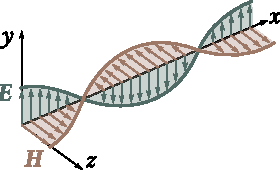
\includegraphics[scale=1]{figures/ch_15/fig_15_1.pdf}
		\caption[]{}
		\label{fig:15_1}
	\end{center}
	\vspace{-0.8cm}
\end{figure}

\section{Điều tra thực nghiệm về sóng điện từ}\label{sec:15_3}

%The first experiments with non-optical electromagnetic waves were conducted in 1888 by the German physicist Heinrich Hertz (1857-1894).
%ertz produced waves with the aid of a vibrator which he had invented.
%The vibrator consisted of two rods separated by a spark gap.
%When a high voltage was fed to the vibrator from an induction coil, a spark jumped through the gap.
%It shorted the latter, and damped electrical oscillations were set up in the vibrator (\fig{15_2}; the chokes shown in the figure were intended to prevent the high-frequency current from branching off into the inductor winding).
%During the time the spark burned, a great number of oscillations were completed.
%They produced a train of electromagnetic waves whose length was approximately twice that of the vibrator.
%By placing vibrators of various length at the focus of a concave parabolic mirror, Hertz obtained directed plane waves whose length ranged from \SIrange{0.6}{10}{\metre}.
Thí nghiệm đầu tiên với sóng điện từ phi quang học được tiến hành trong năm 1888 bởi nhà vật lý người Đức Heinrich Hertz (1857-1894).
Hertz sản xuất sóng với một sự trợ giảng của máy dao động mà do ông ta sáng tạo.
Dao động bao gồm 2 que chia bởi khoảng cách tia lửa.
Khi một điện thế cao được cung cấp cho bộ dao động từ một cuộn dây cảm ứng, một tia lửa lọt vào khe hở.
Nó rút ngắn phần sau và dao động điện tử bị thiệt hại được thiết lập trong thiết bị dao động (\fig{15_2}; các cuộn cảm cho thấy trong hình nhằm ngăn dòng điện cao tần phân nhánh vào cuộc dây cuộn cảm.)
Giữa lúc thời gian tia lửa cháy, mộtlượng lớn số dao động  được hoàn thành.
Họ sản xuất một chuỗi sóng điện từ có độ dài được xấp xỉ gấp đôi chiều dài của máy rung dao động.
Bằng việc đặt máy dao động với độ dài khác nhau tại tiêu điểm của một gương cầu lõm parabol, Hertz đã thu được một sóng phẳng có hướng cùng có chiều dài dao động từ \SIrange{0.6}{10}{\metre}.
\begin{figure}[!htb]
	\begin{center}
		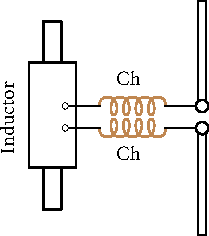
\includegraphics[scale=1]{figures/ch_15/fig_15_2.pdf}
		\caption[]{}
		\label{fig:15_2}
	\end{center}
	\vspace{-0.8cm}
\end{figure}

%When such a vibrator was placed parallel to the electric field strength vector of the wave, oscillations of the current and voltage were produced in it.
%Since the length of the vibrator was equal to $\lambda/2$, the oscillations in it owing to resonance reached such an intensity that they caused small sparks to jump across the spark gap.

Hertz cũng đã nghiên cứu sóng phát ra với sự trợ giúp của một bộ máy rung nửa bước sóng có một khe hở nhỏ ở giữa.
Khi bộ máy rung được đặt song song với vector cường độ điện trường của sóng, các dao động của dòng điện và điện áp được tạo trong đó.
Khi mà độ dài của máy rung là bằng $\lambda/2$, các dao động trong đó tạo ra sự cộng hưởng đạt đến cường độ khiến chúng tạo ra các tia lửa nhỏ nhảy qua các khe tia lửa.

%Hertz reflected and refracted electromagnetic waves with the aid of large metal mirrors and an asphalt prism (over \SI{1}{\metre} in size and with a mass of \SI{1200}{\kilo\gram}).

Hertz cho phản xạ và khúc xạ sóng điện từ với sự hỗ trợ của một chiếc gương kim loại lớn và một lăng kính nhựa (có kính thước trên \SI{1}{\metre} và với khối lượng \SI{1200}{\kilo\gram}).


%He discovered that both these phenomena obey the laws established in optics for light waves.
%By reflecting a running plane wave with the aid of a metal mirror to the opposite direction, Hertz obtained a standing wave.
%The distance between the nodes and antinodes of the wave made it possible to find its length $\lambda$.
%By multiplying $\lambda$ by the frequency of oscillations $\nu$ of the vibrator, the velocity of the electromagnetic waves was determined, and it was found to be close to $c$.

Ông ta khám phá thấy rằng cả hai hiện tượng đều tuân theo định luật trong Quang học đối với sóng ánh sáng.
Bằng cách phản xạ một sóng phẳng với sự hỗ trợ từ một gương kim loại đặt đối diện ngược hướng, Herzt thu được một sóng dừng.
Khoảng cách giữa một nút và bụng sóng giúp tìm được độ dài là $\lambda$.
Nhân $\lambda$ với tần số dao động $\nu$ của bộ máy rung, vận tốc của sóng điện từ được xác định, và nó được tìm thấy là gần với $c$.

%By placing a grate of parallel copper wires in the path of waves, Hertz discovered that the intensity of the waves passing through the grate changes very greatly when the grate is rotated about the beam. When the wires forming the grate were perpendicular to the vector $\vec{E}$, the wave passed through the grate without any hindrance.
%When the wires were arranged parallel to $\vec{E}$, the wave did not pass through the grate.
%Thus, the transverse nature of electromagnetic waves was proved.

Bằng cách đặt một lưới dây đồng đặt song song với đường truyền của sóng, Hertz đã khám phá rằng cường độ sóng truyền qua lưới thay đỏi rất nhiều khi tấm lưới xoay quanh dòng sóng. Khi các dây gộp lại thành lưới vuông góc với với vector $\vec{E}$, sóng truyền qua mà không gặp bất kì trở ngại nào.
Khi các dây được sắp xếp song song với $\vec{E}$, dòng sóng không truyền qua được lưới.
Như vậy, tính chất nằm ngang của sóng điện từ đã được chứng minh.

%Hertz's experiments were continued by the Russian physicist Pyotr Lebedev (1866-1912), who in 1894 obtained electromagnetic waves \SI{6}{\milli\metre} long and studied how they travel in crystals.
%He detected double refraction of the waves (see \sect{19_3}).

Thí nghiệm của Hertz đã được tiếp tục bởi nhà vật lý người Nga Pyotr Lebedev (1866-1912), người mà đã thu được sóng điện từ dài \SI{6}{\milli\metre} và nghiên cứu làm thế nào mà chúng di chuyển trong tinh thể.
Ông ta còn đã phát hiện ra khúc xạ kép trong sóng (xem \sect{19_3}).

%In 1896, the Russian inventor Aleksandr Popov (1859-1905) for the first time in history transmitted a message over a distance of about \SI{250}{\metre} with the aid of electromagnetic waves (the words ``Heinrich Hertz'' were transmitted).
%This laid the foundation of radio engineering.

Trong năm 1896, lần đầu tiên trong lịch sử, nhà phát minh người Nga Aleksandr Popov (1859-1905) đã truyền một tín hiệu với khoảng cách \SI{250}{\metre} nhờ sự trợ giúp của sóng điện từ (từ ``Heinrich Hertz'' đã được truyền gửi).
Điều này đã đặt nền móng cho kĩ thuật vô tuyến.


\section{Năng lượng của sóng điện từ}\label{sec:15_4}

%Electromagnetic waves transfer energy.
%According to \eqn{14_46}, the density of the energy flux can be obtained by multiplying the energy density by the wave velocity.

Sóng điện từ có thể truyền tải năng lượng
Theo như \eqn{14_46}, mật độ dòng năng lượng có thể được quan sát bằng cách nhân mật độ năng lượng với vận tốc sóng.

%The density of the energy of an electromagnetic field $w$ consists of the density of the energy of the electric field [determined by \eqn{4_10}] and that of the energy of the magnetic field [determined
%by \eqn{8_40}]:

Mật độ năng lượng của một trường điện từ $w$ bao gồm mật độ năng lượng của một trường điện [được xác định bằng \eqn{4_10}] và năng lượng của trường từ [được xác định bằng \eqn{8_40}]:

\begin{equation}\label{eq:15_26}
    w = w_E + w_H = \frac{\varepsilon\varepsilon_0 E^2}{2} + \frac{\mu\mu_0 H^2}{2}.
\end{equation}

\noindent
%The vectors $\vec{E}$ and $\vec{H}$ at a given point of space vary in the same phase\footnote{This holds only for a non-conducting medium. The phases of $\vec{E}$ and $\vec{B}$ do not coincide in a conducting medium.}.
%Therefore, \eqn{15_22} giving the relation between the amplitude values of $E$ and $H$ also holds for their instantaneous values.
%It thus follows that the densities of the energy of the electric and magnetic fields of a wave are identical at each moment of time: $w_E = w_H$.
%We can, therefore, write that

Các vector $\vec{E}$ và $\vec{H}$ tại một điểm nhất định trong không gian dao động cùng pha\footnote{Điều này chỉ còn đúng trong môi trường không dẫn điện. Pha của $\vec{E}$ và $\vec{B}$ không trùng nhau trong môi trường dẫn điện.}.
Do đó, \eqn{15_22} cho mối liên hệ giữa các giá trị biên độ của $E$ và $H$ cũng đều giữ một giá trị tức thời của chúng. 
Vì thế cho ta rằng mật độ năng lượng của trường điện và từ của một sóng là như nhau tại mỗi thười điểm $w_E=w_H$. Do đó, chúng ta có thể viết rằng
\begin{equation}\label{eq:15_27}
    w = 2 w_E = \varepsilon\varepsilon_0 E^2.
\end{equation}

%Taking advantage of the fact that $E\sqrt{\varepsilon\varepsilon_0} = H \sqrt{\mu\mu_0}$, we can write \eqn{15_27} in the form

Ta thấy  rằng $E\sqrt{\varepsilon\varepsilon_0} = H \sqrt{\mu\mu_0}$, ta có thể viết \eqn{15_27} ở dạng
\begin{equation*}
    w = \sqrt{\varepsilon\varepsilon_0\mu\mu_0} EH = \frac{1}{v} EH,
\end{equation*}

\noindent
%where $v$ is the velocity of an electromagnetic wave [see \eqn{15_10}].

với $v$ là vận tốc của sóng điện từ [xem \eqn{15_10}]
%Multiplying the expression found for $w$ by the wave velocity $v$, we get the magnitude of the energy flux density vector 

\begin{equation}\label{eq:15_28}
    S = w v = EH.
\end{equation}

\noindent
%The vectors $\vec{E}$ and $\vec{H}$ are mutually perpendicular and form a right-handed system with the direction of propagation of the wave.
%For this reason, the direction of the vector $\vecprod{E}{H}$ coincides with that of energy transfer, and the magnitude of this vector is $EH$.
%Hence, the vector of the density of the electromagnetic energy flux can be written as the vector product of $\vec{E}$ and $\vec{H}$:

2 vector $\vec{E}$ vaf $\vec{H}$ vuông góc với nhau và tạo thành hệ tam diện thuận với theo đường truyền của sóng. Vì lý do này, hướng của vector $\vecprod{E}{H}$ trùng với đường truyền năng lượng và độ lớn của vector nayflaf $EH$. Do đó, vector mật độ dòng năng lượng điện từ có thể được viết dưới dạng tích có hướng vector $\vec{E}$ và $\vec{H}$.

\begin{equation}\label{eq:15_29}
    \vec{S} = \vecprod{E}{H}.
\end{equation}

\noindent
%The vector $\vec{S}$ is known as the \textbf{Poynting vector}.
Vector $\vec{S}$ được biết đến gọi là \textbf{vector Poynting}
%By analogy with \eqn{14_50}, the flux $\Phi$ of electromagnetic energy through surface $\ab{A}{s}$ can be found by integration:
Bằng cách phân tích \eqn{14_50}, năng lượng điện từ $\Phi$ qua mặt phẳng $\ab{A}{s}$ có thể được tìm bằng tích phân: 
\begin{equation}\label{eq:15_30}
    \Phi = \oint_{\ab{A}{s}} \vec{S} \ccdot \ab{\derivec{A}}{s}
\end{equation}
\noindent
%[in \eqn{14_50} the surface area was designated by the symbol $S$; since this symbol is used to designate the Poynting vector, we were forced to introduce the symbol $\ab{A}{s}$ for the surface
area].
[Trong \eqn{14_50} mặt phẳng được kí hiệu tượng trưng bởi kí tự $S$; kí tự này cũng thường được dùng để biểu hiện vector Poynting, vì thế chúng ta sẽ phải dùng đến kí tự $\ab{A}{s}$ cho mặt phẳng].

%Let us consider a portion of a homogeneous cylindrical conductor through which a steady current is flowing (\fig{15_3}) as an example of applying \eqns{15_29}{15_30}.
%We shall first consider that extraneous forces are absent on this portion of the conductor.
%Hence, according to \eqn{5_22}, the following relation is observed at each point of the conductor:

Chúng ta hãy xem một phần của dây dẫn hình trụ đồng chất có dòng điện ổn định chạy qua (\fig{15_3}) như là một ví dụ cho việc áp dụng \eqns{15_29}{15_30}.
Trước tiên, chúng ta xem rằng ngoại lực không có xuất hiện trên phần của dây dẫn.
Vì thề, theo \eqn{5_22}, mối quan hệ trên được quan sát thấy rõ tại mỗi điểm của dây dẫn như sau:
\begin{equation*}
    \vec{j} = \sigma \vec{E} = \frac{1}{\rho} \vec{E}.
\end{equation*}

\begin{figure}[!htb]
	\begin{center}
		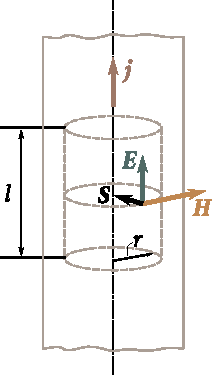
\includegraphics[scale=1]{figures/ch_15/fig_15_3.pdf}
		\caption[]{}
		\label{fig:15_3}
	\end{center}
	\vspace{-0.8cm}
\end{figure}

%The steady current is distributed over the cross section of the conductor with an identical density $\vec{j}$.
%Hence, the electric field within the limits of the portion of the conductor shown in \fig{15_3} will
%be homogeneous.

Dòng ổn định được phân bố trên mặt cách ngang của vật dẫn với mật độ $\vec{j}$ giống hệt nhau.
Do đó, điện trường trong phần giới hạn của dây dẫn trong hình $\fig{15_3}$ sẽ là dạng đồng nhất.


%Let us mentally separate a cylindrical volume of radius $r$ and length $l$ inside the conductor.
%At each point on the side surface of this cylinder, the vector $\vec{H}$ is perpendicular to the vector $\vec{E}$ and is directed tangentially to the surface.
%The magnitude of $\vec{H}$ is $jr/2$ [according to \eqn{7_10}, we have $2\pi rH = j\pi r^2$].
%Thus, the Poynting vector given by \eqn{15_29} is directed toward the axis of the conductor at each point on the surface and has the magnitude $S=EH=Ej r^2/2$.
%Multiplying $S$ by the side surface area of the cylinder $\ab{A}{s}$ equal to $2\pi rl$, we find that the following flux of electromagnetic energy enters the volume we are considering:

Chúng ta hãy tưởng tượng tách riêng một thể tích hình trụ với bán kính $r$ và chiều dài $l$ trong vật dẫn.
Tại mỗi điểm trên mặt bên của hình trụ này, vector $\vec{H}$ vuông góc với vector $\vec{E}$ và có hướng tiếp tuyến với bề mặt.
Độ lớn của $\vec{H}$ là $jr/2$ [ dựa trên phương trình \eqn{7_10}, ta có $2\pi rH = j\pi r^2$].
Vì thế, vector Poynting được cho bởi \eqn{15_29} có hướng về phía trục của dây dẫn tại mỗi điểm trên bề mặt và có độ lớn là $S=EH=Ej r^2/2$.
Nhân giá trị đại lượng $S$ với diện tích bề mặt bên của hình trụ $\ab{A}{s}$ bằng với $2\pi rl$, ta tìm thấy rằng dòng năng lượng điện từ sau đây đi vào thể tích mà ta xem xét tới:

\begin{equation}\label{eq:15_31}
    \Phi = S \ab{A}{s} = \frac{1}{2} Ejr \times 2\pi rl = Ej \times \pi r^2 l = Ej \times V,
\end{equation}

\noindent
%where $V$ is the volume of the cylinder.
Với $V$ là thể tích hình trụ.

%According to \eqn{6_4}, $Ej = pj^2$ is the amount of heat liberated in unit time per unit volume of the conductor.
%Consequently, \eqn{15_31} indicates that the energy liberated in the form of Lenz-Joule heat is supplied to the conductor through its side surface in the form of energy of an electromagnetic field.
%The energy flux gradually weakens with deeper penetration into the conductor (both the Poynting vector and the surface through which the flux passes diminish) as a result of absorption of energy and its conversion into heat.

Theo phương trình \eqn{6_4}, $Ej = pj^2$ là lượng nhiệt tỏa ra trong một đơn vị thời gian trên đơn vị thể tích của vật dẫn.
Kết quả, phương trình chỉ ra rằng năng lượng được giải phóng dưới dạng nhiệt Lenz-Joule, được cung cấp cho dây dẫn qua bề mặt của chính nó theo dạng năng lượng của một trường điện.
Dòng năng lượng dần dần yếu khi thâm nhập sâu vào vật dẫn (cả vector Poynting và bề mặt mà dòng dẫn đi qua đều giảm), theo đó, là kết quả của sự hấp thụ và chuyển đổi nó thành nhiệt.


%Now, let us assume that extraneous forces whose field is homogeneous are exerted within the limits of the portion of the conductor we are considering ($\vec{E}^*=\text{constant}$).
%In this case according to \eqn{5_25}, at each point of the conductor we have

Bây giờ, chúng ta hãy giả sử rằng ngoại lực mà có trường là đồng nhất được tác dụng trong giới hạn của các phần chia vật dẫn mà chúng ta xem xét ($\vec{E}^*=\text{constant}$).
Trong trường hợp đó, dựa vào \eqn{5_25}, theo tại mỗi điểm của vật dẫn ta có
\begin{equation*}
    \vec{j} = \sigma \parenthesis{\vec{E} + \vec{E}^*} = \frac{1}{\rho} \parenthesis{\vec{E} + \vec{E}^*},
\end{equation*}

\noindent
%whence
với
\begin{equation}\label{eq:15_32}
    \vec{E} = \rho \vec{j} - \vec{E}^*.
\end{equation}

\noindent
%We shall consider that the extraneous forces on the portion of the circuit being considered do not hamper the flow of the current, but facilitate it.
%This signifies that the direction of $\vec{E}^*$ coincides with that of $\vec{j}$.
%Let us assume that the relation $\rho j = E^*$ is observed.
%Hence, according to \eqn{15_32}, the electrostatic field strength $\vec{E}$ at each point vanishes, and there is no flux of electromagnetic energy through the side surface.
%In this case, heat is liberated at the expense of the work of the extraneous forces.


Chúng ta nên coi rằng ngoại lực tác dụng lên một phần của mạch điện đang được xem xét không cản trở dòng điện mà ngược lại, tạo điều kiện thuận lợi cho nó.
Điều này biểu thị rằng hướng của $\vec{E}^*$ cùng trùng hướng với $\vec{j}$.
Chúng ta giả sử rằng mối quan hệ $\rho j = E^*$ là đúng.
Vì thế, theo \eqn{15_32}, cường độ trường điện tĩnh với $\vec{E}$ tại mỗi điểm bị triệt tiêu, và không có dòng năng lượng điện từ nào truyền qua mặt bên. 
Trong trường hợp đó, nhiệt được giải phóng do công của các ngoại lực.



%If the relation $E^*>\rho j$ holds, then, as can be seen from \eqn{15_32}, the vector $\vec{E}$ will be directed oppositely to the vector $\vec{j}$.
%In this case, the vectors $\vec{E}$ and $\vec{S}$ will have directions opposite to those shown in \fig{15_3}.
%Hence, instead of flowing in, electromagnetic energy
%flows out through the side surface of the conductor into the space surrounding it.

Nếu mối liên hệ $E^*>\rho j$ đúng, nên, ta có thể thấy từ \eqn{15_32}, vector $\vec{E}$ sẽ có điều hướng ngược lại với vector $\vec{j}$.
Trong trường hợp đó, vectors $\vec{E}$ và $\vec{S}$ sẽ có hướng ngược lại như những gì được cho thấy ở \fig{15_3}.
Khi ấy, thay vì chảy vào, năng lượng điện từ chảy ra qua bề mặt bên của vật dẫn vào trong bề mặt xung quanh chúng.

%In summarizing, we can say that in the closed circuit of a steady current, the energy from the sections where extraneous forces act is transmitted to other sections of the circuit not along the conductors, but through the space surrounding the conductors in the form of a flux of electromagnetic energy characterized by the vector $\vec{S}$.

Tóm tắt lại, chúng ta có thể nói rằng trong một mạch điện kín của một dòng ổn định, năng lượng từ phần tác dụng của ngoại lực được truyền đến các mạch khác trong mạch điện không dọc theo vật dẫn mà qua các không gian bao quanh vật dẫn dưới dạng của một dòng năng lực điện từ được biểu hiện bởi vector $\vec{S}$

\section{Momentum of Electromagnetic Field}\label{sec:15_5}

An electromagnetic wave absorbed in a body imparts a momentum to the body, \ie, exerts a pressure on it.
This can be shown by the following example.
Assume that a plane wave impinges normally onto a flat surface of a weakly conducting body with $\varepsilon$ and $\mu$ equal to unity (\fig{15_4}).
The electric field of the wave produces a current of density $\vec{j} = \sigma\vec{E}$ in the body.
The magnetic field of the wave will act on the current with a force whose value per unit volume of the body can be found by \eqn{6_43}:
\begin{equation*}
    \ab{\vec{F}}{u.v} = \vecprod{j}{B} = \mu_0 (\vecprod{k}{H}).
\end{equation*}

\noindent
The direction of this force, as can be seen from \fig{15_4}, coincides with the direction of propagation of the wave.

\begin{figure}[!htb]
	\begin{center}
		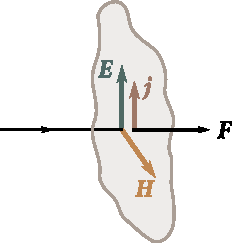
\includegraphics[scale=1]{figures/ch_15/fig_15_4.pdf}
		\caption[]{}
		\label{fig:15_4}
	\end{center}
	\vspace{-0.8cm}
\end{figure}

The momentum
\begin{equation}\label{eq:15_33}
    \deriv{K} = \ab{F}{u.v}\, \deriv{l} = \mu_0 j H\, \deriv{l}
\end{equation}

\noindent
is imparted to a surface layer having a unit area and a thickness of $\deriv{l}$ in unit time (the vectors $\vec{j}$ and $\vec{H}$ are mutually perpendicular).
The energy absorbed in this layer in unit time is
\begin{equation}\label{eq:15_34}
    \deriv{W} = jE\, \deriv{l}.
\end{equation}

\noindent
It is liberated in the form of heat.

The momentum given by \eqn{15_33} and the energy [\eqn{15_34}] are imparted to the layer by the wave.
Let us take their ratio, omitting the differential symbols as superfluous:
\begin{equation*}
    \frac{K}{W} = \mu_0 \frac{H}{E}.
\end{equation*}

\noindent
Taking into account that $\mu_0 H^2=\varepsilon_0 E^2$, we get
\begin{equation*}
    \frac{K}{W} = \sqrt{\varepsilon_0\mu_0} = \frac{1}{c}.
\end{equation*}

\noindent
It thus follows that an electromagnetic wave carrying the energy $W$ has the momentum
\begin{equation}\label{eq:15_35}
    K = \frac{1}{c} W.
\end{equation}

\noindent
The same relation between the energy and the momentum holds for particles with a zero rest mass [see Eq. (8.57) of Vol. I].
This is not surprising because according to quantum notions, an electromagnetic wave is equivalent to a flux of photons, \ie, particles whose mass (we have in mind their rest mass) is zero.

Examination of \eqn{15_35} shows that the density of the momentum (\ie, the momentum of unit volume) of an electromagnetic field is
\begin{equation}\label{eq:15_36}
    \ab{K}{u.v} = \frac{1}{c} w.
\end{equation}

\noindent
The energy density is related to the magnitude of the Poynting vector by the expression $S = wc$. Substituting $S/c$ for $w$ in \eqn{15_36} and taking into account that the directions of the vectors $\vec{K}$ and $\vec{S}$ coincide, we can write that
\begin{equation}\label{eq:15_37}
    \ab{\vec{K}}{u.v} = \frac{1}{c^2} \vec{S} = \frac{1}{c^2} (\vecprod{E}{H}).
\end{equation}

We shall note that when energy of any kind is transferred, the density of the energy flux equals the density of the momentum multiplied by $c^2$.
Let us consider, for example, a collection of particles distributed in space with the density $n$ and flying with a velocity $v$ identical in magnitude and direction.
In this case, the density of the momentum
\begin{equation}\label{eq:15_38}
    \ab{\vec{K}}{u.v} = n \frac{m\vec{v}}{\sqrt{1 - \parenthesis{v^2/c^2}}}.
\end{equation}

\noindent
The particles carry along energy whose density flux $\vec{j}_W$ equals the density of the particle flux multiplied by the energy of one particle:
\begin{equation}\label{eq:15_39}
    \vec{j}_W = n \vec{v} \frac{mc^2}{\sqrt{1 - \parenthesis{v^2/c^2}}}.
\end{equation}

\noindent
It follows from \eqns{15_38}{15_39} that
\begin{equation}\label{eq:15_40}
    \ab{\vec{K}}{u.v} = \frac{1}{c^2} \vec{j}_W.
\end{equation}

Assume that an electromagnetic wave falling normally on a body is completely absorbed by the body.
Hence, a unit of surface area of the body receives in unit time the momentum of the wave enclosed in a cylinder with a base area of unity and an altitude of $c$.
According to \eqn{15_36}, this momentum is $(w/c)c=w$.
At the same time, the momentum imparted to a unit surface area in unit time equals the pressure $p$ on the surface.
Hence, for an absorbing surface, we have $p = w$.
This quantity pulsates with a very high frequency.
We can, therefore, measure its time-averaged value in practice. Thus,
\begin{equation}\label{eq:15_41}
    p = \average{w}.
\end{equation}

\noindent
For an ideally reflecting surface, the pressure will be double this value.

The value of the pressure calculated by \eqn{15_41} is very small.
For example, at a distance of \SI{1}{\metre} from a source of light having an intensity of a million candelas, the pressure is only about \SI{e-7}{\pascal} (about \SI{e-9}{\gf\per\centi\metre\squared}).
Pyotr Lebedev succeeded in measuring the pressure of light.
By carrying out experiments requiring great inventiveness and skill, Lebedev measured the pressure of light on solids in 1900, and on gases in 1910.
The results of the measurements completely agreed with Maxwell's theory.

\section{Dipole Emission}\label{sec:15_6}

An oscillating electric dipole is the simplest system emitting electromagnetic waves.
An example of such a dipole is the system formed by a fixed point charge $+q$ and a point charge $-q$ oscillating near it (\fig{15_5}).
The dipole electric moment of this system varies in time according to the law
\begin{equation}\label{eq:15_42}
    \vec{p} = -q \vec{r} = - ql \hatvec{e} \cos(\omega t) = \ab{\vec{p}}{m} \cos(\omega t),
\end{equation}

\noindent
where $\vec{r}$ is the position vector of the charge $-q$, $l$ the amplitude of oscillations, $\hatvec{e}$ is the unit vector directed along the dipole axis, and $\ab{\vec{p}}{m} =-gl\hatvec{e}$.

\begin{figure}[!htb]
	\begin{minipage}[t]{0.48\linewidth}
		\begin{center}
			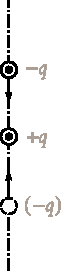
\includegraphics[scale=1]{figures/ch_15/fig_15_5.pdf}
			\caption[]{}
			\label{fig:15_5}
		\end{center}
	\end{minipage}
	\hfill{ }%space{-0.05cm}
	\begin{minipage}[t]{0.48\linewidth}
		\begin{center}
			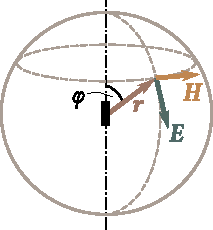
\includegraphics[scale=1]{figures/ch_15/fig_15_6.pdf}
			\caption[]{}
			\label{fig:15_6}
		\end{center}
	\end{minipage}
\vspace{-0.4cm}
\end{figure}

Acquaintance with such an emitting system is especially important in connection with the fact that many questions of the interaction of radiation with a substance can be explained classically proceeding from the notion of atoms as of systems of charges containing electrons that are capable of performing harmonic oscillations about their equilibrium position.

Let us consider the radiation of a dipole whose dimensions are small in comparison with the wavelength ($l\ll\lambda$).
Such a dipole is called \textbf{elementary}.
The pattern of the electromagnetic field in direct proximity to the dipole is very complicated.
It becomes simplified quite greatly in the so-called \textbf{wave zone} of the dipole that begins at distances $r$ considerably exceeding the wavelength ($r\gg\lambda$).
If a wave is propagating in a homogeneous isotropic medium, then its wavefront in the wave zone will be spherical (\fig{15_6}).
The vectors $\vec{E}$ and $\vec{H}$ at each point are mutually perpendicular and are perpendicular to the ray, \ie, to the position vector drawn to the given point from the centre of the dipole.

Let us call sections of the wavefront by planes passing through the dipole axis \textbf{meridians}, and by planes perpendicular to the dipole axis \textbf{parallels}.
We can now say that the vector $\vec{E}$ at each point of a wave zone is directed along a tangent to the meridian, and the vector $\vec{H}$ along a tangent to the parallel.
If we look along the ray $r$, then the instantaneous pattern of the wave will be the same as shown in \fig{15_5}, the only difference being that the amplitude in motion along the ray gradually diminishes.

At each point, the vectors $\vec{E}$ and $\vec{H}$ oscillate according to the law $\cos(\omega t - kr)$.
The amplitudes $\ab{\vec{E}}{m}$ and $\ab{\vec{H}}{m}$ depend on the distance $r$ to the emitter and on the angle a between the direction of the position vector $\vec{r}$ and the dipole axis (see \fig{15_6}).
This dependence has the following form for a vacuum:
\begin{equation*}
    \ab{E}{m} \propto \ab{H}{m} \propto \frac{1}{r} \sin\theta.
\end{equation*}

\noindent
The average value of the density of the energy flux $\average{S}$ is proportional to the product $\ab{E}{m}\ab{H}{m}$, consequently,
\begin{equation}\label{eq:15_43}
    \average{S} \propto \frac{1}{r^2} \sin^2\theta.
\end{equation}

\noindent
A glance at this expression shows that the wave intensity changes along the ray (at $\theta = \text{constant}$) in inverse proportion to the square of the distance from the emitter.
In addition, it depends on the angle $\theta$.
The emission of a dipole is the greatest in directions at right angles to its axis ($\theta = \pi/2$).
There is no emission in the directions coinciding with the axis ($\theta = 0$ and $\pi$).
How the intensity depends on the angle $\theta$ is shown very illustratively with the aid of a \textbf{dipole directional diagram} (\fig{15_7}).
This diagram is constructed so that the length of the segment it intercepts on a ray conducted from the
centre of the dipole gives the intensity of emission at the angle $\theta$.

The corresponding calculations show that the \textbf{radiant power} $P$ of a dipole (\ie, the energy emitted in all directions in unit time) is
proportional to the square of the second time derivative of the dipole moment:
\begin{equation}\label{eq:15_44}
    P \propto \ddot{\vec{p}}^2.
\end{equation}

\begin{figure}[!htb]
	\begin{center}
		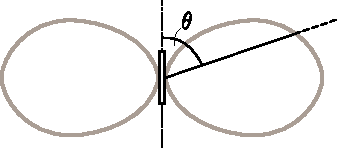
\includegraphics[scale=1]{figures/ch_15/fig_15_7.pdf}
		\caption[]{}
		\label{fig:15_7}
	\end{center}
	\vspace{-0.8cm}
\end{figure}

\noindent
According to \eqn{15_42}, $\ddot{\vec{p}}^2=\ab{p}{m}^2\omega^4\cos^2(\omega t)$.
Introduction of this value into expression \eqref{eq:15_44} yields
\begin{equation}\label{eq:15_45}
    P \propto \ab{p}{m}^2 \omega^4 \cos(\omega t).
\end{equation}

\noindent
Time averaging of this expression gives
\begin{equation}\label{eq:15_46}
    \average{P} \propto \ab{p}{m}^2 \omega^4.
\end{equation}

\noindent
Thus, the average radiant power of a dipole is proportional to the square of the amplitude of the electric dipole moment and to the fourth power of the frequency.
Therefore, at a low frequency, the emission of electrical systems (for instance, industrial frequency alternating current transmission lines) is insignificant.

According to \eqn{15_42}, we have $\ddot{\vec{p}}=-q\ddot{\vec{r}}=-q\vec{a}$, where $\vec{a}$ is the acceleration of an oscillating charge.
Substitution of this expression for $\ddot{\vec{p}}$ in \eqn{15_44} yields\footnote{The constant of proportionality when SI units are used is $\sqrt{\mu_0/\varepsilon_0}/(6\pi c^2)$, and when units of the Gaussian system are used is $2/(3c^3)$.}:
\begin{equation}\label{eq:15_47}
    P \propto q^2 \vec{a}^2.
\end{equation}

\noindent
Expression \eqref{eq:15_47} determines the radiant power not only for oscillations, but also for arbitrary motion of a charge.
A charge travelling with acceleration produces electromagnetic waves, and the radiated power is proportional to the square of the charge and the
square of the acceleration.
For example, the electrons accelerated in a betatron (see \sect{10_5}) lose energy as a result of radiation mainly due to centripetal acceleration $\ab{a}{n}=v^2/r$.
According to expression \eqref{eq:15_47}, the amount of energy lost grows greatly with an increasing velocity of the electrons in the betatron (in proportion to $v^4$).
Hence, the possible acceleration of electrons in a betatron is limited to about \SI{500}{\mega\electronvolt} (at a velocity corresponding to this value, the losses due to radiation become equal to the energy imparted to the electrons by the vortex electric field).

A charge performing harmonic oscillations emits a monochromatic wave with a frequency equal to that of the charge oscillations.
If the acceleration $\vec{a}$ of the charge does not change according to a harmonic law, then the radiation consists of a set of waves of different
frequencies.

According to expression \eqref{eq:15_47}, the intensity vanishes when $\vec{a}=0$.
Consequently, \textit{an electron travelling with a constant velocity does not emit electromagnetic waves}.
This holds, however, only for the case when the velocity of an electron $\ab{v}{el}$ does not exceed the speed of light $\ab{v}{l}=c/\sqrt{\varepsilon\mu}$ in the medium in which the electron is travelling.
When $\ab{v}{el}>\ab{v}{l}$, radiation is observed.
It was discovered in 1934 by the Soviet physicists Sergei Vavilov (1891-1951) and Pavel Cerenkov (born 1904).

% \begin{table}[!b]
% 	\renewcommand{\arraystretch}{1.2}
% 	\caption{}
% 	\vspace{-0.6cm}
% 	\label{table:14_1}
% 	\begin{center}\resizebox{0.65\linewidth}{!}{
% 			\begin{tabular}{lc}
% 				\toprule[1pt]
% 				\textbf{Sound} & \textbf{Loudness level}, \si{\decibel}\\
% 				\midrule[0.5pt]\midrule[0.5pt]
% 				\\
% 				\bottomrule[1pt]
% 			\end{tabular}
% 	}\end{center}
% \end{table}
